\documentclass[1p]{elsarticle_modified}
%\bibliographystyle{elsarticle-num}

%\usepackage[colorlinks]{hyperref}
%\usepackage{abbrmath_seonhwa} %\Abb, \Ascr, \Acal ,\Abf, \Afrak
\usepackage{amsfonts}
\usepackage{amssymb}
\usepackage{amsmath}
\usepackage{amsthm}
\usepackage{scalefnt}
\usepackage{amsbsy}
\usepackage{kotex}
\usepackage{caption}
\usepackage{subfig}
\usepackage{color}
\usepackage{graphicx}
\usepackage{xcolor} %% white, black, red, green, blue, cyan, magenta, yellow
\usepackage{float}
\usepackage{setspace}
\usepackage{hyperref}

\usepackage{tikz}
\usetikzlibrary{arrows}

\usepackage{multirow}
\usepackage{array} % fixed length table
\usepackage{hhline}

%%%%%%%%%%%%%%%%%%%%%
\makeatletter
\renewcommand*\env@matrix[1][\arraystretch]{%
	\edef\arraystretch{#1}%
	\hskip -\arraycolsep
	\let\@ifnextchar\new@ifnextchar
	\array{*\c@MaxMatrixCols c}}
\makeatother %https://tex.stackexchange.com/questions/14071/how-can-i-increase-the-line-spacing-in-a-matrix
%%%%%%%%%%%%%%%

\usepackage[normalem]{ulem}

\newcommand{\msout}[1]{\ifmmode\text{\sout{\ensuremath{#1}}}\else\sout{#1}\fi}
%SOURCE: \msout is \stkout macro in https://tex.stackexchange.com/questions/20609/strikeout-in-math-mode

\newcommand{\cancel}[1]{
	\ifmmode
	{\color{red}\msout{#1}}
	\else
	{\color{red}\sout{#1}}
	\fi
}

\newcommand{\add}[1]{
	{\color{blue}\uwave{#1}}
}

\newcommand{\replace}[2]{
	\ifmmode
	{\color{red}\msout{#1}}{\color{blue}\uwave{#2}}
	\else
	{\color{red}\sout{#1}}{\color{blue}\uwave{#2}}
	\fi
}

\newcommand{\Sol}{\mathcal{S}} %segment
\newcommand{\D}{D} %diagram
\newcommand{\A}{\mathcal{A}} %arc


%%%%%%%%%%%%%%%%%%%%%%%%%%%%%5 test

\def\sl{\operatorname{\textup{SL}}(2,\Cbb)}
\def\psl{\operatorname{\textup{PSL}}(2,\Cbb)}
\def\quan{\mkern 1mu \triangleright \mkern 1mu}

\theoremstyle{definition}
\newtheorem{thm}{Theorem}[section]
\newtheorem{prop}[thm]{Proposition}
\newtheorem{lem}[thm]{Lemma}
\newtheorem{ques}[thm]{Question}
\newtheorem{cor}[thm]{Corollary}
\newtheorem{defn}[thm]{Definition}
\newtheorem{exam}[thm]{Example}
\newtheorem{rmk}[thm]{Remark}
\newtheorem{alg}[thm]{Algorithm}

\newcommand{\I}{\sqrt{-1}}
\begin{document}

%\begin{frontmatter}
%
%\title{Boundary parabolic representations of knots up to 8 crossings}
%
%%% Group authors per affiliation:
%\author{Yunhi Cho} 
%\address{Department of Mathematics, University of Seoul, Seoul, Korea}
%\ead{yhcho@uos.ac.kr}
%
%
%\author{Seonhwa Kim} %\fnref{s_kim}}
%\address{Center for Geometry and Physics, Institute for Basic Science, Pohang, 37673, Korea}
%\ead{ryeona17@ibs.re.kr}
%
%\author{Hyuk Kim}
%\address{Department of Mathematical Sciences, Seoul National University, Seoul 08826, Korea}
%\ead{hyukkim@snu.ac.kr}
%
%\author{Seokbeom Yoon}
%\address{Department of Mathematical Sciences, Seoul National University, Seoul, 08826,  Korea}
%\ead{sbyoon15@snu.ac.kr}
%
%\begin{abstract}
%We find all boundary parabolic representation of knots up to 8 crossings.
%
%\end{abstract}
%\begin{keyword}
%    \MSC[2010] 57M25 
%\end{keyword}
%
%\end{frontmatter}

%\linenumbers
%\tableofcontents
%
\newcommand\colored[1]{\textcolor{white}{\rule[-0.35ex]{0.8em}{1.4ex}}\kern-0.8em\color{red} #1}%
%\newcommand\colored[1]{\textcolor{white}{ #1}\kern-2.17ex	\textcolor{white}{ #1}\kern-1.81ex	\textcolor{white}{ #1}\kern-2.15ex\color{red}#1	}

{\Large $\underline{12n_{0247}~(K12n_{0247})}$}

\setlength{\tabcolsep}{10pt}
\renewcommand{\arraystretch}{1.6}
\vspace{1cm}\begin{tabular}{m{100pt}>{\centering\arraybackslash}m{274pt}}
\multirow{5}{120pt}{
	\centering
	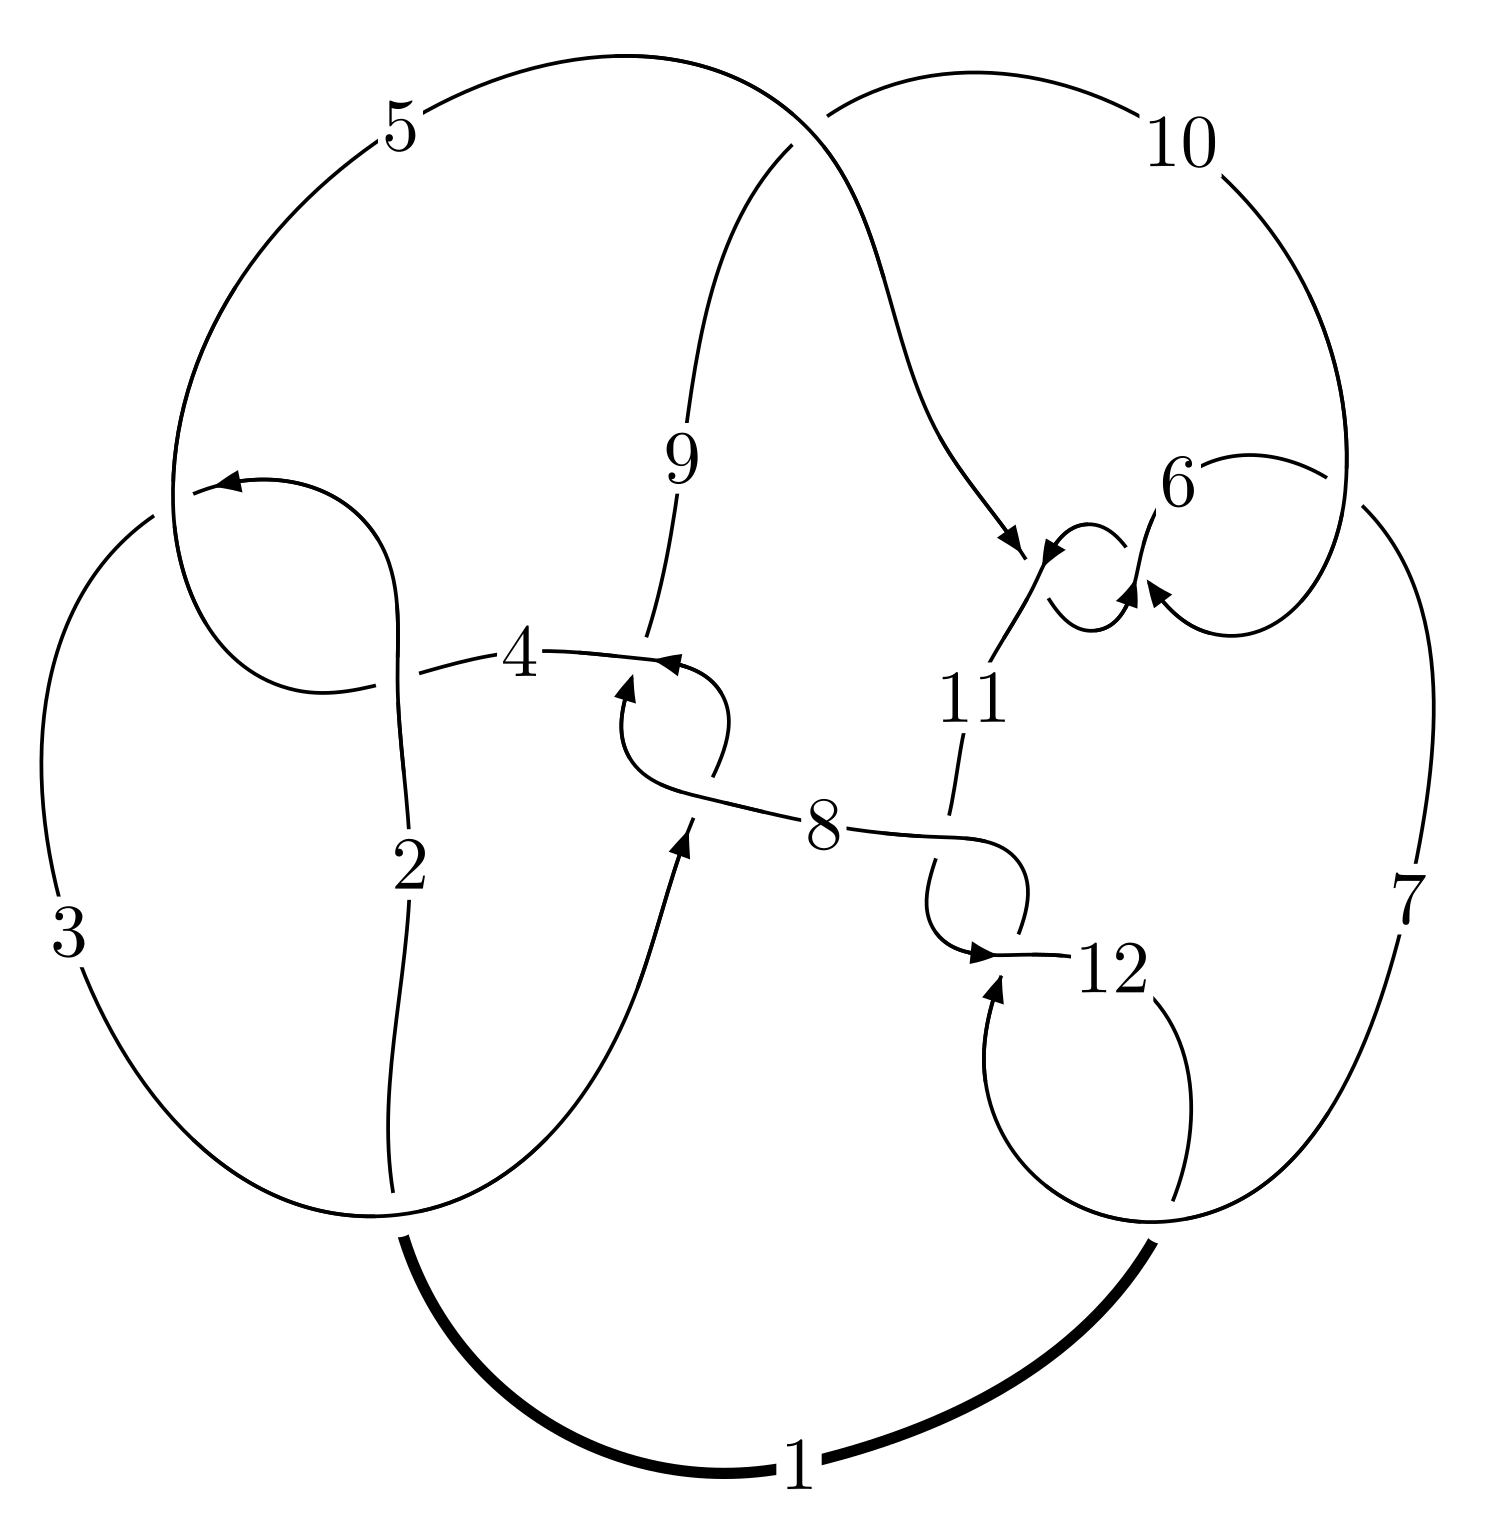
\includegraphics[width=112pt]{../../../GIT/diagram.site/Diagrams/png/2336_12n_0247.png}\\
\ \ \ A knot diagram\footnotemark}&
\allowdisplaybreaks
\textbf{Linearized knot diagam} \\
\cline{2-2}
 &
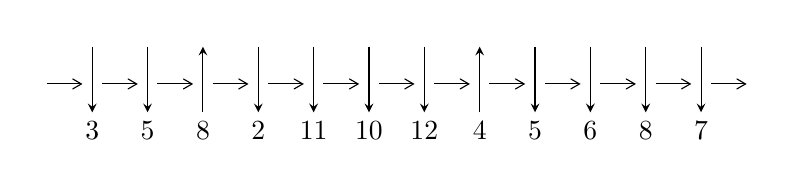
\begin{tikzpicture}[x=20pt, y=17pt]
	% nodes
	\node (C0) at (0, 0) {};
	\node (C1) at (1, 0) {};
	\node (C1U) at (1, +1) {};
	\node (C1D) at (1, -1) {3};

	\node (C2) at (2, 0) {};
	\node (C2U) at (2, +1) {};
	\node (C2D) at (2, -1) {5};

	\node (C3) at (3, 0) {};
	\node (C3U) at (3, +1) {};
	\node (C3D) at (3, -1) {8};

	\node (C4) at (4, 0) {};
	\node (C4U) at (4, +1) {};
	\node (C4D) at (4, -1) {2};

	\node (C5) at (5, 0) {};
	\node (C5U) at (5, +1) {};
	\node (C5D) at (5, -1) {11};

	\node (C6) at (6, 0) {};
	\node (C6U) at (6, +1) {};
	\node (C6D) at (6, -1) {10};

	\node (C7) at (7, 0) {};
	\node (C7U) at (7, +1) {};
	\node (C7D) at (7, -1) {12};

	\node (C8) at (8, 0) {};
	\node (C8U) at (8, +1) {};
	\node (C8D) at (8, -1) {4};

	\node (C9) at (9, 0) {};
	\node (C9U) at (9, +1) {};
	\node (C9D) at (9, -1) {5};

	\node (C10) at (10, 0) {};
	\node (C10U) at (10, +1) {};
	\node (C10D) at (10, -1) {6};

	\node (C11) at (11, 0) {};
	\node (C11U) at (11, +1) {};
	\node (C11D) at (11, -1) {8};

	\node (C12) at (12, 0) {};
	\node (C12U) at (12, +1) {};
	\node (C12D) at (12, -1) {7};
	\node (C13) at (13, 0) {};

	% arrows
	\draw[->,>={angle 60}]
	(C0) edge (C1) (C1) edge (C2) (C2) edge (C3) (C3) edge (C4) (C4) edge (C5) (C5) edge (C6) (C6) edge (C7) (C7) edge (C8) (C8) edge (C9) (C9) edge (C10) (C10) edge (C11) (C11) edge (C12) (C12) edge (C13) ;	\draw[->,>=stealth]
	(C1U) edge (C1D) (C2U) edge (C2D) (C3D) edge (C3U) (C4U) edge (C4D) (C5U) edge (C5D) (C6U) edge (C6D) (C7U) edge (C7D) (C8D) edge (C8U) (C9U) edge (C9D) (C10U) edge (C10D) (C11U) edge (C11D) (C12U) edge (C12D) ;
	\end{tikzpicture} \\
\hhline{~~} \\& 
\textbf{Solving Sequence} \\ \cline{2-2} 
 &
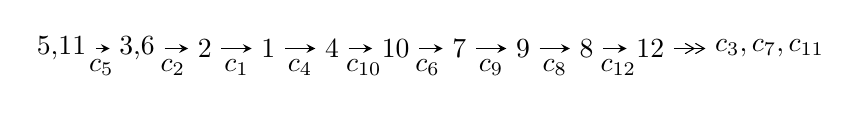
\begin{tikzpicture}[x=23pt, y=7pt]
	% node
	\node (A0) at (-1/8, 0) {5,11};
	\node (A1) at (17/16, 0) {3,6};
	\node (A2) at (17/8, 0) {2};
	\node (A3) at (25/8, 0) {1};
	\node (A4) at (33/8, 0) {4};
	\node (A5) at (41/8, 0) {10};
	\node (A6) at (49/8, 0) {7};
	\node (A7) at (57/8, 0) {9};
	\node (A8) at (65/8, 0) {8};
	\node (A9) at (73/8, 0) {12};
	\node (C1) at (1/2, -1) {$c_{5}$};
	\node (C2) at (13/8, -1) {$c_{2}$};
	\node (C3) at (21/8, -1) {$c_{1}$};
	\node (C4) at (29/8, -1) {$c_{4}$};
	\node (C5) at (37/8, -1) {$c_{10}$};
	\node (C6) at (45/8, -1) {$c_{6}$};
	\node (C7) at (53/8, -1) {$c_{9}$};
	\node (C8) at (61/8, -1) {$c_{8}$};
	\node (C9) at (69/8, -1) {$c_{12}$};
	\node (A10) at (11, 0) {$c_{3},c_{7},c_{11}$};

	% edge
	\draw[->,>=stealth]	
	(A0) edge (A1) (A1) edge (A2) (A2) edge (A3) (A3) edge (A4) (A4) edge (A5) (A5) edge (A6) (A6) edge (A7) (A7) edge (A8) (A8) edge (A9) ;
	\draw[->>,>={angle 60}]	
	(A9) edge (A10);
\end{tikzpicture} \\ 

\end{tabular} \\

\footnotetext{
The image of knot diagram is generated by the software ``\textbf{Draw programme}" developed by Andrew Bartholomew(\url{http://www.layer8.co.uk/maths/draw/index.htm\#Running-draw}), where we modified some parts for our purpose(\url{https://github.com/CATsTAILs/LinksPainter}).
}\phantom \\ \newline 
\centering \textbf{Ideals for irreducible components\footnotemark of $X_{\text{par}}$} 
 
\begin{align*}
I^u_{1}&=\langle 
-3 u^{17}+3 u^{16}+\cdots+32 b+11,\;29 u^{17}+7 u^{16}+\cdots+64 a+79,\;u^{18}+13 u^{16}+\cdots+u-1\rangle \\
I^u_{2}&=\langle 
-345563974 u^{19}-637671531 u^{18}+\cdots+3761745161 b+3368246020,\\
\phantom{I^u_{2}}&\phantom{= \langle  }21843240461 u^{19}+28442594981 u^{18}+\cdots+63949667737 a-48916675361,\\
\phantom{I^u_{2}}&\phantom{= \langle  }u^{20}+2 u^{19}+\cdots-4 u+17\rangle \\
I^u_{3}&=\langle 
b+1,\;u^2+2 a+u+3,\;u^3+2 u-1\rangle \\
I^u_{4}&=\langle 
a^2 u-2 a^2-4 a u+5 b+3 a-5,\;a^3+3 a^2 u-2 a^2- a u- a- u-2,\;u^2+1\rangle \\
I^u_{5}&=\langle 
b+1,\;u^3+u^2+a+u+2,\;u^4+u^3+2 u^2+2 u+1\rangle \\
\\
\end{align*}
\raggedright * 5 irreducible components of $\dim_{\mathbb{C}}=0$, with total 51 representations.\\
\footnotetext{All coefficients of polynomials are rational numbers. But the coefficients are sometimes approximated in decimal forms when there is not enough margin.}
\newpage
\renewcommand{\arraystretch}{1}
\centering \section*{I. $I^u_{1}= \langle -3 u^{17}+3 u^{16}+\cdots+32 b+11,\;29 u^{17}+7 u^{16}+\cdots+64 a+79,\;u^{18}+13 u^{16}+\cdots+u-1 \rangle$}
\flushleft \textbf{(i) Arc colorings}\\
\begin{tabular}{m{7pt} m{180pt} m{7pt} m{180pt} }
\flushright $a_{5}=$&$\begin{pmatrix}1\\0\end{pmatrix}$ \\
\flushright $a_{11}=$&$\begin{pmatrix}0\\u\end{pmatrix}$ \\
\flushright $a_{3}=$&$\begin{pmatrix}-0.453125 u^{17}-0.109375 u^{16}+\cdots-5.84375 u-1.23438\\0.0937500 u^{17}-0.0937500 u^{16}+\cdots-0.812500 u-0.343750\end{pmatrix}$ \\
\flushright $a_{6}=$&$\begin{pmatrix}1\\u^2\end{pmatrix}$ \\
\flushright $a_{2}=$&$\begin{pmatrix}-0.359375 u^{17}-0.203125 u^{16}+\cdots-6.65625 u-1.57813\\0.0937500 u^{17}-0.0937500 u^{16}+\cdots-0.812500 u-0.343750\end{pmatrix}$ \\
\flushright $a_{1}=$&$\begin{pmatrix}- u^3-2 u\\-\frac{1}{8} u^{16}-\frac{3}{2} u^{14}+\cdots+\frac{7}{8} u+\frac{1}{8}\end{pmatrix}$ \\
\flushright $a_{4}=$&$\begin{pmatrix}-0.640625 u^{17}-0.296875 u^{16}+\cdots-5.59375 u-1.17188\\-0.406250 u^{17}-0.0937500 u^{16}+\cdots-0.562500 u-0.843750\end{pmatrix}$ \\
\flushright $a_{10}=$&$\begin{pmatrix}u\\u^3+u\end{pmatrix}$ \\
\flushright $a_{7}=$&$\begin{pmatrix}u^2+1\\u^4+2 u^2\end{pmatrix}$ \\
\flushright $a_{9}=$&$\begin{pmatrix}u^3+2 u\\u^3+u\end{pmatrix}$ \\
\flushright $a_{8}=$&$\begin{pmatrix}-1\\\frac{1}{8} u^{17}+\frac{3}{2} u^{15}+\cdots-\frac{23}{8} u^2-\frac{1}{8} u\end{pmatrix}$ \\
\flushright $a_{12}=$&$\begin{pmatrix}- u\\-\frac{1}{8} u^{16}-\frac{3}{2} u^{14}+\cdots+\frac{7}{8} u+\frac{1}{8}\end{pmatrix}$\\&\end{tabular}
\flushleft \textbf{(ii) Obstruction class $= -1$}\\~\\
\flushleft \textbf{(iii) Cusp Shapes $= \frac{229}{128} u^{17}-\frac{33}{128} u^{16}+\cdots+\frac{427}{64} u-\frac{505}{128}$}\\~\\
\newpage\renewcommand{\arraystretch}{1}
\flushleft \textbf{(iv) u-Polynomials at the component}\newline \\
\begin{tabular}{m{50pt}|m{274pt}}
Crossings & \hspace{64pt}u-Polynomials at each crossing \\
\hline $$\begin{aligned}c_{1}\end{aligned}$$&$\begin{aligned}
&u^{18}+4 u^{17}+\cdots+257 u+16
\end{aligned}$\\
\hline $$\begin{aligned}c_{2},c_{4}\end{aligned}$$&$\begin{aligned}
&u^{18}-4 u^{17}+\cdots+13 u-4
\end{aligned}$\\
\hline $$\begin{aligned}c_{3},c_{8}\end{aligned}$$&$\begin{aligned}
&u^{18}+3 u^{17}+\cdots+232 u+32
\end{aligned}$\\
\hline $$\begin{aligned}c_{5},c_{6},c_{7}\\c_{10},c_{11},c_{12}\end{aligned}$$&$\begin{aligned}
&u^{18}+13 u^{16}+\cdots+u-1
\end{aligned}$\\
\hline $$\begin{aligned}c_{9}\end{aligned}$$&$\begin{aligned}
&u^{18}-6 u^{17}+\cdots-256 u-256
\end{aligned}$\\
\hline
\end{tabular}\\~\\
\newpage\renewcommand{\arraystretch}{1}
\flushleft \textbf{(v) Riley Polynomials at the component}\newline \\
\begin{tabular}{m{50pt}|m{274pt}}
Crossings & \hspace{64pt}Riley Polynomials at each crossing \\
\hline $$\begin{aligned}c_{1}\end{aligned}$$&$\begin{aligned}
&y^{18}+24 y^{17}+\cdots-22945 y+256
\end{aligned}$\\
\hline $$\begin{aligned}c_{2},c_{4}\end{aligned}$$&$\begin{aligned}
&y^{18}-4 y^{17}+\cdots-257 y+16
\end{aligned}$\\
\hline $$\begin{aligned}c_{3},c_{8}\end{aligned}$$&$\begin{aligned}
&y^{18}-21 y^{17}+\cdots-10560 y+1024
\end{aligned}$\\
\hline $$\begin{aligned}c_{5},c_{6},c_{7}\\c_{10},c_{11},c_{12}\end{aligned}$$&$\begin{aligned}
&y^{18}+26 y^{17}+\cdots-11 y+1
\end{aligned}$\\
\hline $$\begin{aligned}c_{9}\end{aligned}$$&$\begin{aligned}
&y^{18}+26 y^{17}+\cdots-98304 y+65536
\end{aligned}$\\
\hline
\end{tabular}\\~\\
\newpage\flushleft \textbf{(vi) Complex Volumes and Cusp Shapes}
$$\begin{array}{c|c|c}  
\text{Solutions to }I^u_{1}& \I (\text{vol} + \sqrt{-1}CS) & \text{Cusp shape}\\
 \hline 
\begin{aligned}
u &= \phantom{-}0.513277 + 0.615531 I \\
a &= \phantom{-}0.69273 - 1.30024 I \\
b &= \phantom{-}0.926284 + 0.896765 I\end{aligned}
 & \phantom{-}5.03715 - 4.73308 I & -6.17449 + 6.98654 I \\ \hline\begin{aligned}
u &= \phantom{-}0.513277 - 0.615531 I \\
a &= \phantom{-}0.69273 + 1.30024 I \\
b &= \phantom{-}0.926284 - 0.896765 I\end{aligned}
 & \phantom{-}5.03715 + 4.73308 I & -6.17449 - 6.98654 I \\ \hline\begin{aligned}
u &= \phantom{-}0.322723 + 0.641738 I \\
a &= -0.511493 + 0.469718 I \\
b &= \phantom{-}0.907757 - 0.852129 I\end{aligned}
 & \phantom{-}5.02936 + 1.72315 I & -6.30423 + 2.05854 I \\ \hline\begin{aligned}
u &= \phantom{-}0.322723 - 0.641738 I \\
a &= -0.511493 - 0.469718 I \\
b &= \phantom{-}0.907757 + 0.852129 I\end{aligned}
 & \phantom{-}5.02936 - 1.72315 I & -6.30423 - 2.05854 I \\ \hline\begin{aligned}
u &= \phantom{-}0.20594 + 1.41832 I \\
a &= \phantom{-}0.550117 - 0.463999 I \\
b &= \phantom{-}0.820288 + 0.298128 I\end{aligned}
 & \phantom{-}8.20719 - 5.81488 I & \phantom{-}1.58758 + 8.21476 I \\ \hline\begin{aligned}
u &= \phantom{-}0.20594 - 1.41832 I \\
a &= \phantom{-}0.550117 + 0.463999 I \\
b &= \phantom{-}0.820288 - 0.298128 I\end{aligned}
 & \phantom{-}8.20719 + 5.81488 I & \phantom{-}1.58758 - 8.21476 I \\ \hline\begin{aligned}
u &= -0.559591\phantom{ +0.000000I} \\
a &= \phantom{-}1.08527\phantom{ +0.000000I} \\
b &= \phantom{-}0.320915\phantom{ +0.000000I}\end{aligned}
 & -1.10260\phantom{ +0.000000I} & -8.67790\phantom{ +0.000000I} \\ \hline\begin{aligned}
u &= -0.274931 + 0.275799 I \\
a &= \phantom{-}0.85438 - 1.34319 I \\
b &= -0.518997 + 0.250386 I\end{aligned}
 & -0.591534 + 0.915522 I & -8.76058 - 7.51611 I \\ \hline\begin{aligned}
u &= -0.274931 - 0.275799 I \\
a &= \phantom{-}0.85438 + 1.34319 I \\
b &= -0.518997 - 0.250386 I\end{aligned}
 & -0.591534 - 0.915522 I & -8.76058 + 7.51611 I \\ \hline\begin{aligned}
u &= -0.04969 + 1.63263 I \\
a &= -0.017613 - 0.874719 I \\
b &= -1.39382 + 0.44407 I\end{aligned}
 & \phantom{-}9.47411 + 1.71565 I & -2.49915 - 0.68525 I\\
 \hline 
 \end{array}$$\newpage$$\begin{array}{c|c|c}  
\text{Solutions to }I^u_{1}& \I (\text{vol} + \sqrt{-1}CS) & \text{Cusp shape}\\
 \hline 
\begin{aligned}
u &= -0.04969 - 1.63263 I \\
a &= -0.017613 + 0.874719 I \\
b &= -1.39382 - 0.44407 I\end{aligned}
 & \phantom{-}9.47411 - 1.71565 I & -2.49915 + 0.68525 I \\ \hline\begin{aligned}
u &= -0.39884 + 1.63329 I \\
a &= \phantom{-}0.30757 + 1.53003 I \\
b &= \phantom{-}1.25592 - 0.96097 I\end{aligned}
 & -19.6148 + 12.8943 I & -2.00648 - 5.58395 I \\ \hline\begin{aligned}
u &= -0.39884 - 1.63329 I \\
a &= \phantom{-}0.30757 - 1.53003 I \\
b &= \phantom{-}1.25592 + 0.96097 I\end{aligned}
 & -19.6148 - 12.8943 I & -2.00648 + 5.58395 I \\ \hline\begin{aligned}
u &= \phantom{-}0.16134 + 1.67469 I \\
a &= \phantom{-}0.135382 + 1.232190 I \\
b &= -0.453358 - 1.088430 I\end{aligned}
 & \phantom{-}12.98160 - 4.39049 I & -1.06537 + 2.81298 I \\ \hline\begin{aligned}
u &= \phantom{-}0.16134 - 1.67469 I \\
a &= \phantom{-}0.135382 - 1.232190 I \\
b &= -0.453358 + 1.088430 I\end{aligned}
 & \phantom{-}12.98160 + 4.39049 I & -1.06537 - 2.81298 I \\ \hline\begin{aligned}
u &= \phantom{-}0.264194\phantom{ +0.000000I} \\
a &= -3.30167\phantom{ +0.000000I} \\
b &= -1.07735\phantom{ +0.000000I}\end{aligned}
 & -2.03333\phantom{ +0.000000I} & \phantom{-}1.10900\phantom{ +0.000000I} \\ \hline\begin{aligned}
u &= -0.33212 + 1.72012 I \\
a &= -0.652868 - 0.820297 I \\
b &= \phantom{-}0.83415 + 1.30011 I\end{aligned}
 & -18.1326 + 4.7805 I & -0.86783 - 1.39495 I \\ \hline\begin{aligned}
u &= -0.33212 - 1.72012 I \\
a &= -0.652868 + 0.820297 I \\
b &= \phantom{-}0.83415 - 1.30011 I\end{aligned}
 & -18.1326 - 4.7805 I & -0.86783 + 1.39495 I\\
 \hline 
 \end{array}$$\newpage\newpage\renewcommand{\arraystretch}{1}
\centering \section*{II. $I^u_{2}= \langle -3.46\times10^{8} u^{19}-6.38\times10^{8} u^{18}+\cdots+3.76\times10^{9} b+3.37\times10^{9},\;2.18\times10^{10} u^{19}+2.84\times10^{10} u^{18}+\cdots+6.39\times10^{10} a-4.89\times10^{10},\;u^{20}+2 u^{19}+\cdots-4 u+17 \rangle$}
\flushleft \textbf{(i) Arc colorings}\\
\begin{tabular}{m{7pt} m{180pt} m{7pt} m{180pt} }
\flushright $a_{5}=$&$\begin{pmatrix}1\\0\end{pmatrix}$ \\
\flushright $a_{11}=$&$\begin{pmatrix}0\\u\end{pmatrix}$ \\
\flushright $a_{3}=$&$\begin{pmatrix}-0.341569 u^{19}-0.444765 u^{18}+\cdots-6.80195 u+0.764925\\0.0918627 u^{19}+0.169515 u^{18}+\cdots+1.48236 u-0.895395\end{pmatrix}$ \\
\flushright $a_{6}=$&$\begin{pmatrix}1\\u^2\end{pmatrix}$ \\
\flushright $a_{2}=$&$\begin{pmatrix}-0.249707 u^{19}-0.275251 u^{18}+\cdots-5.31959 u-0.130470\\0.0918627 u^{19}+0.169515 u^{18}+\cdots+1.48236 u-0.895395\end{pmatrix}$ \\
\flushright $a_{1}=$&$\begin{pmatrix}0.0321030 u^{19}+0.154890 u^{18}+\cdots-1.20856 u+1.30329\\0.0116403 u^{19}+0.0303223 u^{18}+\cdots-0.600017 u+0.446055\end{pmatrix}$ \\
\flushright $a_{4}=$&$\begin{pmatrix}-0.274136 u^{19}-0.394973 u^{18}+\cdots-4.73485 u-0.948502\\0.105172 u^{19}+0.211195 u^{18}+\cdots+1.77125 u-1.07336\end{pmatrix}$ \\
\flushright $a_{10}=$&$\begin{pmatrix}u\\u^3+u\end{pmatrix}$ \\
\flushright $a_{7}=$&$\begin{pmatrix}u^2+1\\u^4+2 u^2\end{pmatrix}$ \\
\flushright $a_{9}=$&$\begin{pmatrix}u^3+2 u\\u^3+u\end{pmatrix}$ \\
\flushright $a_{8}=$&$\begin{pmatrix}0.0540994 u^{19}+0.0710831 u^{18}+\cdots+0.210536 u+1.58028\\-0.0628232 u^{19}-0.0347199 u^{18}+\cdots-1.06815 u+1.63097\end{pmatrix}$ \\
\flushright $a_{12}=$&$\begin{pmatrix}-0.0217078 u^{19}+0.0194076 u^{18}+\cdots-3.38491 u+1.15498\\-0.0538109 u^{19}-0.135483 u^{18}+\cdots-0.176349 u-0.148305\end{pmatrix}$\\&\end{tabular}
\flushleft \textbf{(ii) Obstruction class $= -1$}\\~\\
\flushleft \textbf{(iii) Cusp Shapes $= \frac{687646779}{3761745161} u^{19}+\frac{3390901343}{3761745161} u^{18}+\cdots+\frac{12009014830}{3761745161} u-\frac{7942008906}{3761745161}$}\\~\\
\newpage\renewcommand{\arraystretch}{1}
\flushleft \textbf{(iv) u-Polynomials at the component}\newline \\
\begin{tabular}{m{50pt}|m{274pt}}
Crossings & \hspace{64pt}u-Polynomials at each crossing \\
\hline $$\begin{aligned}c_{1}\end{aligned}$$&$\begin{aligned}
&(u^{10}+u^9+10 u^8+11 u^7+26 u^6+30 u^5+u^4-14 u^3+3 u^2-2 u+1)^2
\end{aligned}$\\
\hline $$\begin{aligned}c_{2},c_{4}\end{aligned}$$&$\begin{aligned}
&(u^{10}-3 u^9+4 u^8+u^7-6 u^6+6 u^5+u^4-2 u^3+3 u^2-2 u+1)^2
\end{aligned}$\\
\hline $$\begin{aligned}c_{3},c_{8}\end{aligned}$$&$\begin{aligned}
&(u^{10}- u^9-7 u^8+8 u^7+13 u^6-14 u^5-2 u^4-2 u^3+13 u^2-12 u+4)^2
\end{aligned}$\\
\hline $$\begin{aligned}c_{5},c_{6},c_{7}\\c_{10},c_{11},c_{12}\end{aligned}$$&$\begin{aligned}
&u^{20}+2 u^{19}+\cdots-4 u+17
\end{aligned}$\\
\hline $$\begin{aligned}c_{9}\end{aligned}$$&$\begin{aligned}
&(u^{10}+2 u^9+\cdots-21 u+17)^{2}
\end{aligned}$\\
\hline
\end{tabular}\\~\\
\newpage\renewcommand{\arraystretch}{1}
\flushleft \textbf{(v) Riley Polynomials at the component}\newline \\
\begin{tabular}{m{50pt}|m{274pt}}
Crossings & \hspace{64pt}Riley Polynomials at each crossing \\
\hline $$\begin{aligned}c_{1}\end{aligned}$$&$\begin{aligned}
&(y^{10}+19 y^9+\cdots+2 y+1)^{2}
\end{aligned}$\\
\hline $$\begin{aligned}c_{2},c_{4}\end{aligned}$$&$\begin{aligned}
&(y^{10}- y^9+10 y^8-11 y^7+26 y^6-30 y^5+y^4+14 y^3+3 y^2+2 y+1)^2
\end{aligned}$\\
\hline $$\begin{aligned}c_{3},c_{8}\end{aligned}$$&$\begin{aligned}
&(y^{10}-15 y^9+\cdots-40 y+16)^{2}
\end{aligned}$\\
\hline $$\begin{aligned}c_{5},c_{6},c_{7}\\c_{10},c_{11},c_{12}\end{aligned}$$&$\begin{aligned}
&y^{20}+18 y^{19}+\cdots+1480 y+289
\end{aligned}$\\
\hline $$\begin{aligned}c_{9}\end{aligned}$$&$\begin{aligned}
&(y^{10}+26 y^9+\cdots+2925 y+289)^{2}
\end{aligned}$\\
\hline
\end{tabular}\\~\\
\newpage\flushleft \textbf{(vi) Complex Volumes and Cusp Shapes}
$$\begin{array}{c|c|c}  
\text{Solutions to }I^u_{2}& \I (\text{vol} + \sqrt{-1}CS) & \text{Cusp shape}\\
 \hline 
\begin{aligned}
u &= \phantom{-}0.598226 + 0.786865 I \\
a &= \phantom{-}0.005030 + 0.155416 I \\
b &= -0.076965 - 0.657059 I\end{aligned}
 & \phantom{-}4.43566 - 1.46073 I & -1.34069 + 3.28644 I \\ \hline\begin{aligned}
u &= \phantom{-}0.598226 - 0.786865 I \\
a &= \phantom{-}0.005030 - 0.155416 I \\
b &= -0.076965 + 0.657059 I\end{aligned}
 & \phantom{-}4.43566 + 1.46073 I & -1.34069 - 3.28644 I \\ \hline\begin{aligned}
u &= -0.014778 + 1.179270 I \\
a &= \phantom{-}0.90480 + 1.65650 I \\
b &= -1.016000 - 0.211624 I\end{aligned}
 & \phantom{-}1.39065 - 0.79591 I & -8.77960 - 0.81155 I \\ \hline\begin{aligned}
u &= -0.014778 - 1.179270 I \\
a &= \phantom{-}0.90480 - 1.65650 I \\
b &= -1.016000 + 0.211624 I\end{aligned}
 & \phantom{-}1.39065 + 0.79591 I & -8.77960 + 0.81155 I \\ \hline\begin{aligned}
u &= -1.077400 + 0.591320 I \\
a &= \phantom{-}0.927031 + 0.754940 I \\
b &= \phantom{-}1.12142 - 1.03617 I\end{aligned}
 & \phantom{-}12.6890 + 7.4068 I & -3.25674 - 4.41038 I \\ \hline\begin{aligned}
u &= -1.077400 - 0.591320 I \\
a &= \phantom{-}0.927031 - 0.754940 I \\
b &= \phantom{-}1.12142 + 1.03617 I\end{aligned}
 & \phantom{-}12.6890 - 7.4068 I & -3.25674 + 4.41038 I \\ \hline\begin{aligned}
u &= -1.033740 + 0.754404 I \\
a &= -0.0441939 - 0.0300635 I \\
b &= \phantom{-}0.98889 + 1.13481 I\end{aligned}
 & \phantom{-}13.15130 - 0.50253 I & -2.50299 - 0.08773 I \\ \hline\begin{aligned}
u &= -1.033740 - 0.754404 I \\
a &= -0.0441939 + 0.0300635 I \\
b &= \phantom{-}0.98889 - 1.13481 I\end{aligned}
 & \phantom{-}13.15130 + 0.50253 I & -2.50299 + 0.08773 I \\ \hline\begin{aligned}
u &= -0.220229 + 1.263180 I \\
a &= \phantom{-}0.634760 + 0.673705 I \\
b &= \phantom{-}0.482659 - 0.410726 I\end{aligned}
 & \phantom{-}2.87696 + 2.81207 I & -3.11998 - 4.64391 I \\ \hline\begin{aligned}
u &= -0.220229 - 1.263180 I \\
a &= \phantom{-}0.634760 - 0.673705 I \\
b &= \phantom{-}0.482659 + 0.410726 I\end{aligned}
 & \phantom{-}2.87696 - 2.81207 I & -3.11998 + 4.64391 I\\
 \hline 
 \end{array}$$\newpage$$\begin{array}{c|c|c}  
\text{Solutions to }I^u_{2}& \I (\text{vol} + \sqrt{-1}CS) & \text{Cusp shape}\\
 \hline 
\begin{aligned}
u &= \phantom{-}0.661189 + 0.252982 I \\
a &= \phantom{-}1.093740 + 0.337893 I \\
b &= \phantom{-}0.482659 + 0.410726 I\end{aligned}
 & \phantom{-}2.87696 - 2.81207 I & -3.11998 + 4.64391 I \\ \hline\begin{aligned}
u &= \phantom{-}0.661189 - 0.252982 I \\
a &= \phantom{-}1.093740 - 0.337893 I \\
b &= \phantom{-}0.482659 - 0.410726 I\end{aligned}
 & \phantom{-}2.87696 + 2.81207 I & -3.11998 - 4.64391 I \\ \hline\begin{aligned}
u &= -0.208282 + 0.650238 I \\
a &= -3.22497 - 1.66304 I \\
b &= -1.016000 + 0.211624 I\end{aligned}
 & \phantom{-}1.39065 + 0.79591 I & -8.77960 + 0.81155 I \\ \hline\begin{aligned}
u &= -0.208282 - 0.650238 I \\
a &= -3.22497 + 1.66304 I \\
b &= -1.016000 - 0.211624 I\end{aligned}
 & \phantom{-}1.39065 - 0.79591 I & -8.77960 - 0.81155 I \\ \hline\begin{aligned}
u &= \phantom{-}0.065595 + 1.361450 I \\
a &= \phantom{-}0.719320 - 1.166450 I \\
b &= -0.076965 + 0.657059 I\end{aligned}
 & \phantom{-}4.43566 + 1.46073 I & -1.34069 - 3.28644 I \\ \hline\begin{aligned}
u &= \phantom{-}0.065595 - 1.361450 I \\
a &= \phantom{-}0.719320 + 1.166450 I \\
b &= -0.076965 - 0.657059 I\end{aligned}
 & \phantom{-}4.43566 - 1.46073 I & -1.34069 + 3.28644 I \\ \hline\begin{aligned}
u &= \phantom{-}0.17643 + 1.61460 I \\
a &= -0.17553 - 1.65533 I \\
b &= \phantom{-}1.12142 + 1.03617 I\end{aligned}
 & \phantom{-}12.6890 - 7.4068 I & -3.25674 + 4.41038 I \\ \hline\begin{aligned}
u &= \phantom{-}0.17643 - 1.61460 I \\
a &= -0.17553 + 1.65533 I \\
b &= \phantom{-}1.12142 - 1.03617 I\end{aligned}
 & \phantom{-}12.6890 + 7.4068 I & -3.25674 - 4.41038 I \\ \hline\begin{aligned}
u &= \phantom{-}0.05299 + 1.63807 I \\
a &= -0.63412 + 1.33106 I \\
b &= \phantom{-}0.98889 - 1.13481 I\end{aligned}
 & \phantom{-}13.15130 + 0.50253 I & -2.50299 + 0.08773 I \\ \hline\begin{aligned}
u &= \phantom{-}0.05299 - 1.63807 I \\
a &= -0.63412 - 1.33106 I \\
b &= \phantom{-}0.98889 + 1.13481 I\end{aligned}
 & \phantom{-}13.15130 - 0.50253 I & -2.50299 - 0.08773 I\\
 \hline 
 \end{array}$$\newpage\newpage\renewcommand{\arraystretch}{1}
\centering \section*{III. $I^u_{3}= \langle b+1,\;u^2+2 a+u+3,\;u^3+2 u-1 \rangle$}
\flushleft \textbf{(i) Arc colorings}\\
\begin{tabular}{m{7pt} m{180pt} m{7pt} m{180pt} }
\flushright $a_{5}=$&$\begin{pmatrix}1\\0\end{pmatrix}$ \\
\flushright $a_{11}=$&$\begin{pmatrix}0\\u\end{pmatrix}$ \\
\flushright $a_{3}=$&$\begin{pmatrix}-\frac{1}{2} u^2-\frac{1}{2} u-\frac{3}{2}\\-1\end{pmatrix}$ \\
\flushright $a_{6}=$&$\begin{pmatrix}1\\u^2\end{pmatrix}$ \\
\flushright $a_{2}=$&$\begin{pmatrix}-\frac{1}{2} u^2-\frac{1}{2} u-\frac{5}{2}\\-1\end{pmatrix}$ \\
\flushright $a_{1}=$&$\begin{pmatrix}-1\\0\end{pmatrix}$ \\
\flushright $a_{4}=$&$\begin{pmatrix}-\frac{1}{2} u^2-\frac{1}{2} u-\frac{3}{2}\\-1\end{pmatrix}$ \\
\flushright $a_{10}=$&$\begin{pmatrix}u\\- u+1\end{pmatrix}$ \\
\flushright $a_{7}=$&$\begin{pmatrix}u^2+1\\u\end{pmatrix}$ \\
\flushright $a_{9}=$&$\begin{pmatrix}1\\- u+1\end{pmatrix}$ \\
\flushright $a_{8}=$&$\begin{pmatrix}1\\- u+1\end{pmatrix}$ \\
\flushright $a_{12}=$&$\begin{pmatrix}- u\\u^2\end{pmatrix}$\\&\end{tabular}
\flushleft \textbf{(ii) Obstruction class $= 1$}\\~\\
\flushleft \textbf{(iii) Cusp Shapes $= -\frac{25}{4} u^2-\frac{11}{4} u-\frac{71}{4}$}\\~\\
\newpage\renewcommand{\arraystretch}{1}
\flushleft \textbf{(iv) u-Polynomials at the component}\newline \\
\begin{tabular}{m{50pt}|m{274pt}}
Crossings & \hspace{64pt}u-Polynomials at each crossing \\
\hline $$\begin{aligned}c_{1},c_{2}\end{aligned}$$&$\begin{aligned}
&(u-1)^3
\end{aligned}$\\
\hline $$\begin{aligned}c_{3},c_{8}\end{aligned}$$&$\begin{aligned}
&u^3
\end{aligned}$\\
\hline $$\begin{aligned}c_{4}\end{aligned}$$&$\begin{aligned}
&(u+1)^3
\end{aligned}$\\
\hline $$\begin{aligned}c_{5},c_{6},c_{7}\end{aligned}$$&$\begin{aligned}
&u^3+2 u-1
\end{aligned}$\\
\hline $$\begin{aligned}c_{9}\end{aligned}$$&$\begin{aligned}
&u^3+3 u^2+5 u+2
\end{aligned}$\\
\hline $$\begin{aligned}c_{10},c_{11},c_{12}\end{aligned}$$&$\begin{aligned}
&u^3+2 u+1
\end{aligned}$\\
\hline
\end{tabular}\\~\\
\newpage\renewcommand{\arraystretch}{1}
\flushleft \textbf{(v) Riley Polynomials at the component}\newline \\
\begin{tabular}{m{50pt}|m{274pt}}
Crossings & \hspace{64pt}Riley Polynomials at each crossing \\
\hline $$\begin{aligned}c_{1},c_{2},c_{4}\end{aligned}$$&$\begin{aligned}
&(y-1)^3
\end{aligned}$\\
\hline $$\begin{aligned}c_{3},c_{8}\end{aligned}$$&$\begin{aligned}
&y^3
\end{aligned}$\\
\hline $$\begin{aligned}c_{5},c_{6},c_{7}\\c_{10},c_{11},c_{12}\end{aligned}$$&$\begin{aligned}
&y^3+4 y^2+4 y-1
\end{aligned}$\\
\hline $$\begin{aligned}c_{9}\end{aligned}$$&$\begin{aligned}
&y^3+y^2+13 y-4
\end{aligned}$\\
\hline
\end{tabular}\\~\\
\newpage\flushleft \textbf{(vi) Complex Volumes and Cusp Shapes}
$$\begin{array}{c|c|c}  
\text{Solutions to }I^u_{3}& \I (\text{vol} + \sqrt{-1}CS) & \text{Cusp shape}\\
 \hline 
\begin{aligned}
u &= -0.22670 + 1.46771 I \\
a &= -0.335258 - 0.401127 I \\
b &= -1.00000\phantom{ +0.000000I}\end{aligned}
 & \phantom{-}7.79580 + 5.13794 I & -3.98417 + 0.12290 I \\ \hline\begin{aligned}
u &= -0.22670 - 1.46771 I \\
a &= -0.335258 + 0.401127 I \\
b &= -1.00000\phantom{ +0.000000I}\end{aligned}
 & \phantom{-}7.79580 - 5.13794 I & -3.98417 - 0.12290 I \\ \hline\begin{aligned}
u &= \phantom{-}0.453398\phantom{ +0.000000I} \\
a &= -1.82948\phantom{ +0.000000I} \\
b &= -1.00000\phantom{ +0.000000I}\end{aligned}
 & -2.43213\phantom{ +0.000000I} & -20.2820\phantom{ +0.000000I}\\
 \hline 
 \end{array}$$\newpage\newpage\renewcommand{\arraystretch}{1}
\centering \section*{IV. $I^u_{4}= \langle a^2 u-2 a^2-4 a u+5 b+3 a-5,\;a^3+3 a^2 u-2 a^2- a u- a- u-2,\;u^2+1 \rangle$}
\flushleft \textbf{(i) Arc colorings}\\
\begin{tabular}{m{7pt} m{180pt} m{7pt} m{180pt} }
\flushright $a_{5}=$&$\begin{pmatrix}1\\0\end{pmatrix}$ \\
\flushright $a_{11}=$&$\begin{pmatrix}0\\u\end{pmatrix}$ \\
\flushright $a_{3}=$&$\begin{pmatrix}a\\-\frac{1}{5} a^2 u+\frac{4}{5} a u+\cdots-\frac{3}{5} a+1\end{pmatrix}$ \\
\flushright $a_{6}=$&$\begin{pmatrix}1\\-1\end{pmatrix}$ \\
\flushright $a_{2}=$&$\begin{pmatrix}-\frac{1}{5} a^2 u+\frac{4}{5} a u+\cdots+\frac{2}{5} a+1\\-\frac{1}{5} a^2 u+\frac{4}{5} a u+\cdots-\frac{3}{5} a+1\end{pmatrix}$ \\
\flushright $a_{1}=$&$\begin{pmatrix}- u\\-\frac{2}{5} a^2 u-\frac{2}{5} a u+\cdots+\frac{4}{5} a+2\end{pmatrix}$ \\
\flushright $a_{4}=$&$\begin{pmatrix}\frac{3}{5} a^2 u-\frac{1}{5} a^2-\frac{7}{5} a u-\frac{1}{5} a\\-\frac{1}{5} a^2 u-\frac{3}{5} a^2-\frac{6}{5} a u+\frac{7}{5} a\end{pmatrix}$ \\
\flushright $a_{10}=$&$\begin{pmatrix}u\\0\end{pmatrix}$ \\
\flushright $a_{7}=$&$\begin{pmatrix}0\\-1\end{pmatrix}$ \\
\flushright $a_{9}=$&$\begin{pmatrix}u\\0\end{pmatrix}$ \\
\flushright $a_{8}=$&$\begin{pmatrix}-1\\\frac{1}{5} a^2 u-\frac{4}{5} a u+\cdots-\frac{2}{5} a^2-\frac{2}{5} a\end{pmatrix}$ \\
\flushright $a_{12}=$&$\begin{pmatrix}- u\\-\frac{2}{5} a^2 u-\frac{2}{5} a u+\cdots+\frac{4}{5} a+2\end{pmatrix}$\\&\end{tabular}
\flushleft \textbf{(ii) Obstruction class $= 1$}\\~\\
\flushleft \textbf{(iii) Cusp Shapes $= -\frac{4}{5} a^2 u+\frac{8}{5} a^2+\frac{16}{5} a u-\frac{12}{5} a$}\\~\\
\newpage\renewcommand{\arraystretch}{1}
\flushleft \textbf{(iv) u-Polynomials at the component}\newline \\
\begin{tabular}{m{50pt}|m{274pt}}
Crossings & \hspace{64pt}u-Polynomials at each crossing \\
\hline $$\begin{aligned}c_{1}\end{aligned}$$&$\begin{aligned}
&(u^3- u^2+2 u-1)^2
\end{aligned}$\\
\hline $$\begin{aligned}c_{2}\end{aligned}$$&$\begin{aligned}
&(u^3+u^2-1)^2
\end{aligned}$\\
\hline $$\begin{aligned}c_{3},c_{8}\end{aligned}$$&$\begin{aligned}
&u^6-3 u^4+2 u^2+1
\end{aligned}$\\
\hline $$\begin{aligned}c_{4}\end{aligned}$$&$\begin{aligned}
&(u^3- u^2+1)^2
\end{aligned}$\\
\hline $$\begin{aligned}c_{5},c_{6},c_{7}\\c_{10},c_{11},c_{12}\end{aligned}$$&$\begin{aligned}
&(u^2+1)^3
\end{aligned}$\\
\hline $$\begin{aligned}c_{9}\end{aligned}$$&$\begin{aligned}
&u^6
\end{aligned}$\\
\hline
\end{tabular}\\~\\
\newpage\renewcommand{\arraystretch}{1}
\flushleft \textbf{(v) Riley Polynomials at the component}\newline \\
\begin{tabular}{m{50pt}|m{274pt}}
Crossings & \hspace{64pt}Riley Polynomials at each crossing \\
\hline $$\begin{aligned}c_{1}\end{aligned}$$&$\begin{aligned}
&(y^3+3 y^2+2 y-1)^2
\end{aligned}$\\
\hline $$\begin{aligned}c_{2},c_{4}\end{aligned}$$&$\begin{aligned}
&(y^3- y^2+2 y-1)^2
\end{aligned}$\\
\hline $$\begin{aligned}c_{3},c_{8}\end{aligned}$$&$\begin{aligned}
&(y^3-3 y^2+2 y+1)^2
\end{aligned}$\\
\hline $$\begin{aligned}c_{5},c_{6},c_{7}\\c_{10},c_{11},c_{12}\end{aligned}$$&$\begin{aligned}
&(y+1)^6
\end{aligned}$\\
\hline $$\begin{aligned}c_{9}\end{aligned}$$&$\begin{aligned}
&y^6
\end{aligned}$\\
\hline
\end{tabular}\\~\\
\newpage\flushleft \textbf{(vi) Complex Volumes and Cusp Shapes}
$$\begin{array}{c|c|c}  
\text{Solutions to }I^u_{4}& \I (\text{vol} + \sqrt{-1}CS) & \text{Cusp shape}\\
 \hline 
\begin{aligned}
u &= \phantom{-0.000000 -}1.000000 I \\
a &= \phantom{-}0.684841 - 1.082500 I \\
b &= \phantom{-}0.877439 + 0.744862 I\end{aligned}
 & \phantom{-}6.31400 - 2.82812 I & -0.49024 + 2.97945 I \\ \hline\begin{aligned}
u &= \phantom{-0.000000 -}1.000000 I \\
a &= -0.439718 + 0.407221 I \\
b &= \phantom{-}0.877439 - 0.744862 I\end{aligned}
 & \phantom{-}6.31400 + 2.82812 I & -0.49024 - 2.97945 I \\ \hline\begin{aligned}
u &= \phantom{-0.000000 -}1.000000 I \\
a &= \phantom{-}1.75488 - 2.32472 I \\
b &= -0.754878\phantom{ +0.000000I}\end{aligned}
 & \phantom{-}2.17641\phantom{ +0.000000I} & -7.01951 + 0. I\phantom{ +0.000000I} \\ \hline\begin{aligned}
u &= \phantom{-0.000000 } -1.000000 I \\
a &= \phantom{-}0.684841 + 1.082500 I \\
b &= \phantom{-}0.877439 - 0.744862 I\end{aligned}
 & \phantom{-}6.31400 + 2.82812 I & -0.49024 - 2.97945 I \\ \hline\begin{aligned}
u &= \phantom{-0.000000 } -1.000000 I \\
a &= -0.439718 - 0.407221 I \\
b &= \phantom{-}0.877439 + 0.744862 I\end{aligned}
 & \phantom{-}6.31400 - 2.82812 I & -0.49024 + 2.97945 I \\ \hline\begin{aligned}
u &= \phantom{-0.000000 } -1.000000 I \\
a &= \phantom{-}1.75488 + 2.32472 I \\
b &= -0.754878\phantom{ +0.000000I}\end{aligned}
 & \phantom{-}2.17641\phantom{ +0.000000I} & -7.01951 + 0. I\phantom{ +0.000000I}\\
 \hline 
 \end{array}$$\newpage\newpage\renewcommand{\arraystretch}{1}
\centering \section*{V. $I^u_{5}= \langle b+1,\;u^3+u^2+a+u+2,\;u^4+u^3+2 u^2+2 u+1 \rangle$}
\flushleft \textbf{(i) Arc colorings}\\
\begin{tabular}{m{7pt} m{180pt} m{7pt} m{180pt} }
\flushright $a_{5}=$&$\begin{pmatrix}1\\0\end{pmatrix}$ \\
\flushright $a_{11}=$&$\begin{pmatrix}0\\u\end{pmatrix}$ \\
\flushright $a_{3}=$&$\begin{pmatrix}- u^3- u^2- u-2\\-1\end{pmatrix}$ \\
\flushright $a_{6}=$&$\begin{pmatrix}1\\u^2\end{pmatrix}$ \\
\flushright $a_{2}=$&$\begin{pmatrix}- u^3- u^2- u-3\\-1\end{pmatrix}$ \\
\flushright $a_{1}=$&$\begin{pmatrix}-1\\0\end{pmatrix}$ \\
\flushright $a_{4}=$&$\begin{pmatrix}- u^3- u^2- u-2\\-1\end{pmatrix}$ \\
\flushright $a_{10}=$&$\begin{pmatrix}u\\u^3+u\end{pmatrix}$ \\
\flushright $a_{7}=$&$\begin{pmatrix}u^2+1\\- u^3-2 u-1\end{pmatrix}$ \\
\flushright $a_{9}=$&$\begin{pmatrix}u^3+2 u\\u^3+u\end{pmatrix}$ \\
\flushright $a_{8}=$&$\begin{pmatrix}u^3+2 u\\u^3+u\end{pmatrix}$ \\
\flushright $a_{12}=$&$\begin{pmatrix}-2 u^3- u^2-3 u-3\\- u^3- u^2- u-2\end{pmatrix}$\\&\end{tabular}
\flushleft \textbf{(ii) Obstruction class $= 1$}\\~\\
\flushleft \textbf{(iii) Cusp Shapes $= -4 u^3-4 u-9$}\\~\\
\newpage\renewcommand{\arraystretch}{1}
\flushleft \textbf{(iv) u-Polynomials at the component}\newline \\
\begin{tabular}{m{50pt}|m{274pt}}
Crossings & \hspace{64pt}u-Polynomials at each crossing \\
\hline $$\begin{aligned}c_{1},c_{2}\end{aligned}$$&$\begin{aligned}
&(u-1)^4
\end{aligned}$\\
\hline $$\begin{aligned}c_{3},c_{8}\end{aligned}$$&$\begin{aligned}
&u^4
\end{aligned}$\\
\hline $$\begin{aligned}c_{4}\end{aligned}$$&$\begin{aligned}
&(u+1)^4
\end{aligned}$\\
\hline $$\begin{aligned}c_{5},c_{6},c_{7}\end{aligned}$$&$\begin{aligned}
&u^4+u^3+2 u^2+2 u+1
\end{aligned}$\\
\hline $$\begin{aligned}c_{9}\end{aligned}$$&$\begin{aligned}
&(u^2- u+1)^2
\end{aligned}$\\
\hline $$\begin{aligned}c_{10},c_{11},c_{12}\end{aligned}$$&$\begin{aligned}
&u^4- u^3+2 u^2-2 u+1
\end{aligned}$\\
\hline
\end{tabular}\\~\\
\newpage\renewcommand{\arraystretch}{1}
\flushleft \textbf{(v) Riley Polynomials at the component}\newline \\
\begin{tabular}{m{50pt}|m{274pt}}
Crossings & \hspace{64pt}Riley Polynomials at each crossing \\
\hline $$\begin{aligned}c_{1},c_{2},c_{4}\end{aligned}$$&$\begin{aligned}
&(y-1)^4
\end{aligned}$\\
\hline $$\begin{aligned}c_{3},c_{8}\end{aligned}$$&$\begin{aligned}
&y^4
\end{aligned}$\\
\hline $$\begin{aligned}c_{5},c_{6},c_{7}\\c_{10},c_{11},c_{12}\end{aligned}$$&$\begin{aligned}
&y^4+3 y^3+2 y^2+1
\end{aligned}$\\
\hline $$\begin{aligned}c_{9}\end{aligned}$$&$\begin{aligned}
&(y^2+y+1)^2
\end{aligned}$\\
\hline
\end{tabular}\\~\\
\newpage\flushleft \textbf{(vi) Complex Volumes and Cusp Shapes}
$$\begin{array}{c|c|c}  
\text{Solutions to }I^u_{5}& \I (\text{vol} + \sqrt{-1}CS) & \text{Cusp shape}\\
 \hline 
\begin{aligned}
u &= -0.621744 + 0.440597 I \\
a &= -1.69244 - 0.31815 I \\
b &= -1.00000\phantom{ +0.000000I}\end{aligned}
 & \phantom{-}1.64493 + 2.02988 I & -7.00000 - 3.46410 I \\ \hline\begin{aligned}
u &= -0.621744 - 0.440597 I \\
a &= -1.69244 + 0.31815 I \\
b &= -1.00000\phantom{ +0.000000I}\end{aligned}
 & \phantom{-}1.64493 - 2.02988 I & -7.00000 + 3.46410 I \\ \hline\begin{aligned}
u &= \phantom{-}0.121744 + 1.306620 I \\
a &= \phantom{-}0.192440 + 0.547877 I \\
b &= -1.00000\phantom{ +0.000000I}\end{aligned}
 & \phantom{-}1.64493 - 2.02988 I & -7.00000 + 3.46410 I \\ \hline\begin{aligned}
u &= \phantom{-}0.121744 - 1.306620 I \\
a &= \phantom{-}0.192440 - 0.547877 I \\
b &= -1.00000\phantom{ +0.000000I}\end{aligned}
 & \phantom{-}1.64493 + 2.02988 I & -7.00000 - 3.46410 I\\
 \hline 
 \end{array}$$\newpage
\newpage\renewcommand{\arraystretch}{1}
\centering \section*{ VI. u-Polynomials}
\begin{tabular}{m{50pt}|m{274pt}}
Crossings & \hspace{64pt}u-Polynomials at each crossing \\
\hline $$\begin{aligned}c_{1}\end{aligned}$$&$\begin{aligned}
&(u-1)^7(u^3- u^2+2 u-1)^2\\
&\cdot(u^{10}+u^9+10 u^8+11 u^7+26 u^6+30 u^5+u^4-14 u^3+3 u^2-2 u+1)^2\\
&\cdot(u^{18}+4 u^{17}+\cdots+257 u+16)
\end{aligned}$\\
\hline $$\begin{aligned}c_{2}\end{aligned}$$&$\begin{aligned}
&(u-1)^7(u^3+u^2-1)^2\\
&\cdot(u^{10}-3 u^9+4 u^8+u^7-6 u^6+6 u^5+u^4-2 u^3+3 u^2-2 u+1)^2\\
&\cdot(u^{18}-4 u^{17}+\cdots+13 u-4)
\end{aligned}$\\
\hline $$\begin{aligned}c_{3},c_{8}\end{aligned}$$&$\begin{aligned}
&u^7(u^6-3 u^4+2 u^2+1)\\
&\cdot(u^{10}- u^9-7 u^8+8 u^7+13 u^6-14 u^5-2 u^4-2 u^3+13 u^2-12 u+4)^2\\
&\cdot(u^{18}+3 u^{17}+\cdots+232 u+32)
\end{aligned}$\\
\hline $$\begin{aligned}c_{4}\end{aligned}$$&$\begin{aligned}
&(u+1)^7(u^3- u^2+1)^2\\
&\cdot(u^{10}-3 u^9+4 u^8+u^7-6 u^6+6 u^5+u^4-2 u^3+3 u^2-2 u+1)^2\\
&\cdot(u^{18}-4 u^{17}+\cdots+13 u-4)
\end{aligned}$\\
\hline $$\begin{aligned}c_{5},c_{6},c_{7}\end{aligned}$$&$\begin{aligned}
&((u^2+1)^3)(u^3+2 u-1)(u^4+u^3+\cdots+2 u+1)(u^{18}+13 u^{16}+\cdots+u-1)\\
&\cdot(u^{20}+2 u^{19}+\cdots-4 u+17)
\end{aligned}$\\
\hline $$\begin{aligned}c_{9}\end{aligned}$$&$\begin{aligned}
&u^6(u^2- u+1)^2(u^{3}+3 u^{2}+5 u+2)(u^{10}+2 u^{9}+\cdots-21 u+17)^{2}\\
&\cdot(u^{18}-6 u^{17}+\cdots-256 u-256)
\end{aligned}$\\
\hline $$\begin{aligned}c_{10},c_{11},c_{12}\end{aligned}$$&$\begin{aligned}
&((u^2+1)^3)(u^3+2 u+1)(u^4- u^3+\cdots-2 u+1)(u^{18}+13 u^{16}+\cdots+u-1)\\
&\cdot(u^{20}+2 u^{19}+\cdots-4 u+17)
\end{aligned}$\\
\hline
\end{tabular}\newpage\renewcommand{\arraystretch}{1}
\centering \section*{ VII. Riley Polynomials}
\begin{tabular}{m{50pt}|m{274pt}}
Crossings & \hspace{64pt}Riley Polynomials at each crossing \\
\hline $$\begin{aligned}c_{1}\end{aligned}$$&$\begin{aligned}
&((y-1)^7)(y^3+3 y^2+2 y-1)^2(y^{10}+19 y^9+\cdots+2 y+1)^{2}\\
&\cdot(y^{18}+24 y^{17}+\cdots-22945 y+256)
\end{aligned}$\\
\hline $$\begin{aligned}c_{2},c_{4}\end{aligned}$$&$\begin{aligned}
&(y-1)^7(y^3- y^2+2 y-1)^2\\
&\cdot(y^{10}- y^9+10 y^8-11 y^7+26 y^6-30 y^5+y^4+14 y^3+3 y^2+2 y+1)^2\\
&\cdot(y^{18}-4 y^{17}+\cdots-257 y+16)
\end{aligned}$\\
\hline $$\begin{aligned}c_{3},c_{8}\end{aligned}$$&$\begin{aligned}
&y^7(y^3-3 y^2+2 y+1)^2(y^{10}-15 y^9+\cdots-40 y+16)^{2}\\
&\cdot(y^{18}-21 y^{17}+\cdots-10560 y+1024)
\end{aligned}$\\
\hline $$\begin{aligned}c_{5},c_{6},c_{7}\\c_{10},c_{11},c_{12}\end{aligned}$$&$\begin{aligned}
&(y+1)^6(y^3+4 y^2+4 y-1)(y^4+3 y^3+2 y^2+1)\\
&\cdot(y^{18}+26 y^{17}+\cdots-11 y+1)(y^{20}+18 y^{19}+\cdots+1480 y+289)
\end{aligned}$\\
\hline $$\begin{aligned}c_{9}\end{aligned}$$&$\begin{aligned}
&y^6(y^2+y+1)^2(y^{3}+y^{2}+13 y-4)(y^{10}+26 y^{9}+\cdots+2925 y+289)^{2}\\
&\cdot(y^{18}+26 y^{17}+\cdots-98304 y+65536)
\end{aligned}$\\
\hline
\end{tabular}
\vskip 2pc
\end{document}